%-------------------------------PPT Title-------------------------------------
\title{\rm{LINUX}环境、命令与\rm{GNU}软件编译}
%-----------------------------------------------------------------------------

%----------------------------Author & Date------------------------------------
%\author[\textrm{Jun\_Jiang}]{姜\;\;骏\inst{}} %[]{} (optional, use only with lots of authors)
%% - Give the names in the same order as the appear in the paper.
%% - Use the \inst{?} command only if the authors have different
%%   affiliation.
\institute[BCC]{\inst{}%
 \vskip -20pt 北京市计算中心 云平台}
\date[\today] % (optional, should be abbreviation of conference name)
{	%{\fontsize{6.2pt}{4.2pt}\selectfont{\textcolor{blue}{E-mail:~}\url{jiangjun@bcc.ac.cn}}}
\vskip 45 pt {\fontsize{8.2pt}{6.2pt}\selectfont{%中国科学院\;\;理论物理所% 报告地点
	\vskip 5 pt \textrm{2021.07.13}}}
}

%% - Either use conference name or its abbreviation
%% - Not really information to the audience, more for people (including
%%   yourself) who are reading the slides onlin%%   yourself) who are reading the slides onlin%%   yourself) who are reading the slides onlineee
%%%%%%%%%%%%%%%%%%%%%%%%%%%%%%%%%%%%%%%%%%%%%%%%%%%%%%%%%%%%%%%%%%%%%%%%%%%%%%%%%%%%%%%%%%%%%%%%%%%%%%%%%%%%%%%%%%%%%

\subject{}
% This is only inserted into the PDF information catalog. Can be left
% out.
%\maketitle
\frame
{
%	\frametitle{\fontsize{9.5pt}{5.2pt}\selectfont{\textcolor{orange}{“高通量并发式材料计算算法与软件”年度检查}}}
\titlepage
}
%-----------------------------------------------------------------------------

%------------------------------------------------------------------------------列出全文 outline ---------------------------------------------------------------------------------
\small
\section{\rm{Linux}操作系统概述}
\frame
{
	\frametitle{\textrm{Linux}操作系统简介}
	\textrm{Linux}是\textrm{1991}年由芬兰的\textrm{Linus~Benedic~Torvalds}设计的、可运行在微机上的\textrm{UNIX}系统\footnote{\fontsize{5.0pt}{4.2pt}\selectfont{\textrm{UNIX}是一种多任务分时操作系统,以``核\textrm{kernel}''-``壳(shell)''结构为特色,最初是由\textrm{AT\&T~Bell}实验室开发的,具有安全可靠、使用方便、开放性和可移植性号等优点,可在各类机型上广泛使用。\textrm{Internet}就是在\textrm{UNIX}基础上发展起来的。}}。

	\textrm{Linux}基于\textrm{POSIX}和\textrm{UNIX}的多用户、多任务、支持多线程和多\textrm{CPU}的操作系统。它能运行主要的\textrm{UNIX}工具软件、应用程序和网络协议。它支持32位和64位硬件。\textrm{Linux}继承了\textrm{UNIX}以网络为核心的设计思想,是\underline{\textcolor{blue}{性能稳定}}的\underline{\textcolor{blue}{多用户}}网络操作系统。
	\vskip 12pt
\begin{minipage}{0.58\textwidth}
\textrm{Linux}操作系统的特点:
\begin{itemize}
	\item 完全免费
	\item 支持多用户、多任务工作方式
	\item 界面友好
	\item 支持多种硬件平台
\end{itemize}
\end{minipage}
\begin{minipage}{0.40\textwidth}
\begin{figure}[h!]
\centering
\vspace{-1.5pt}

\includegraphics[height=1.3in,width=1.1in,viewport=0 0 380 450,clip]{Figures/Linux-logo.jpg}
%\caption{\textrm{The wave-particle duality and Photoelectric effect}}
\label{Linux-Logo}
\end{figure}
\end{minipage}
}

\frame
{
	\frametitle{为什么使用\textrm{Linux}}
	\begin{itemize}
\setlength{\itemsep}{10pt}
		\item 开放性和良好的可移植性
			\begin{enumerate}
				\item \textrm{Linux}是完全\textcolor{purple}{开源}和\textcolor{purple}{免费}的
				\item \textrm{Linux}使用 \textrm{C}语言对硬件资源的管理,可移植性好
			\end{enumerate}
\item 丰富的软件开发环境,系统高效
	\begin{enumerate}
		\item 多种高级语言
		\item 强有力的调试手段
		\item 方便的文本编辑和应用程序
	\end{enumerate}
\item 自然科学与工程技术研究软件中的大部分是在\textrm{Linux}环境下开发与使用的
	\end{itemize}
	\textcolor{red}{用户知道自己想要什么,也明白自己在做什么,并会为自己的行为负责}
}

\frame
{
	\frametitle{\textrm{Linux}的常见发行版本}
	\begin{itemize}
		\item 基于RMP系列
\begin{figure}[h!]
\centering
\vspace*{-0.2in}
\subfigure[\textrm{Redhat}]{
\label{fig:Redhat}

\includegraphics[height=0.9in,width=0.85in,viewport=0 0 350 350,clip]{Figures/Linux_redhat-logo.jpg}}
\subfigure[\textrm{Fedora}]{
\label{fig:Fedra}

\includegraphics[height=0.9in,width=0.85in,viewport=0 0 275 275,clip]{Figures/Linux_fedora-logo.jpg}}
\subfigure[\textrm{CentOS}]{
\label{fig:CentOS}

\includegraphics[height=0.9in,width=0.85in,viewport=150 0 650 470,clip]{Figures/Linux_centos-logo.jpg}}
%\caption{\tiny \textrm{The Band-structure from Molecular-orbital.}}%
\label{RPM-seroes}
\end{figure} 
		\item 基于Debian系列
\begin{figure}[h!]
\centering
\vspace*{-0.1in}
\subfigure[\textrm{Debian}]{
\label{fig:Debian}

\includegraphics[height=0.9in,width=1.75in,viewport=0 0 415 235,clip]{Figures/Linux_debian-logo.jpg}}
\subfigure[\textrm{Ubuntu}]{
\label{fig:Ubuntu}

\includegraphics[height=0.9in,width=0.95in,viewport=0 0 280 280,clip]{Figures/Linux_ubuntu-logo.jpg}}
%\caption{\tiny \textrm{The Band-structure from Molecular-orbital.}}%
\label{debian-seroes}
\end{figure} 
	\end{itemize}
}

\frame
{
	\frametitle{\textrm{Linux}发行版本的关系}
\begin{figure}[h!]
\centering
\vspace{21.5pt}
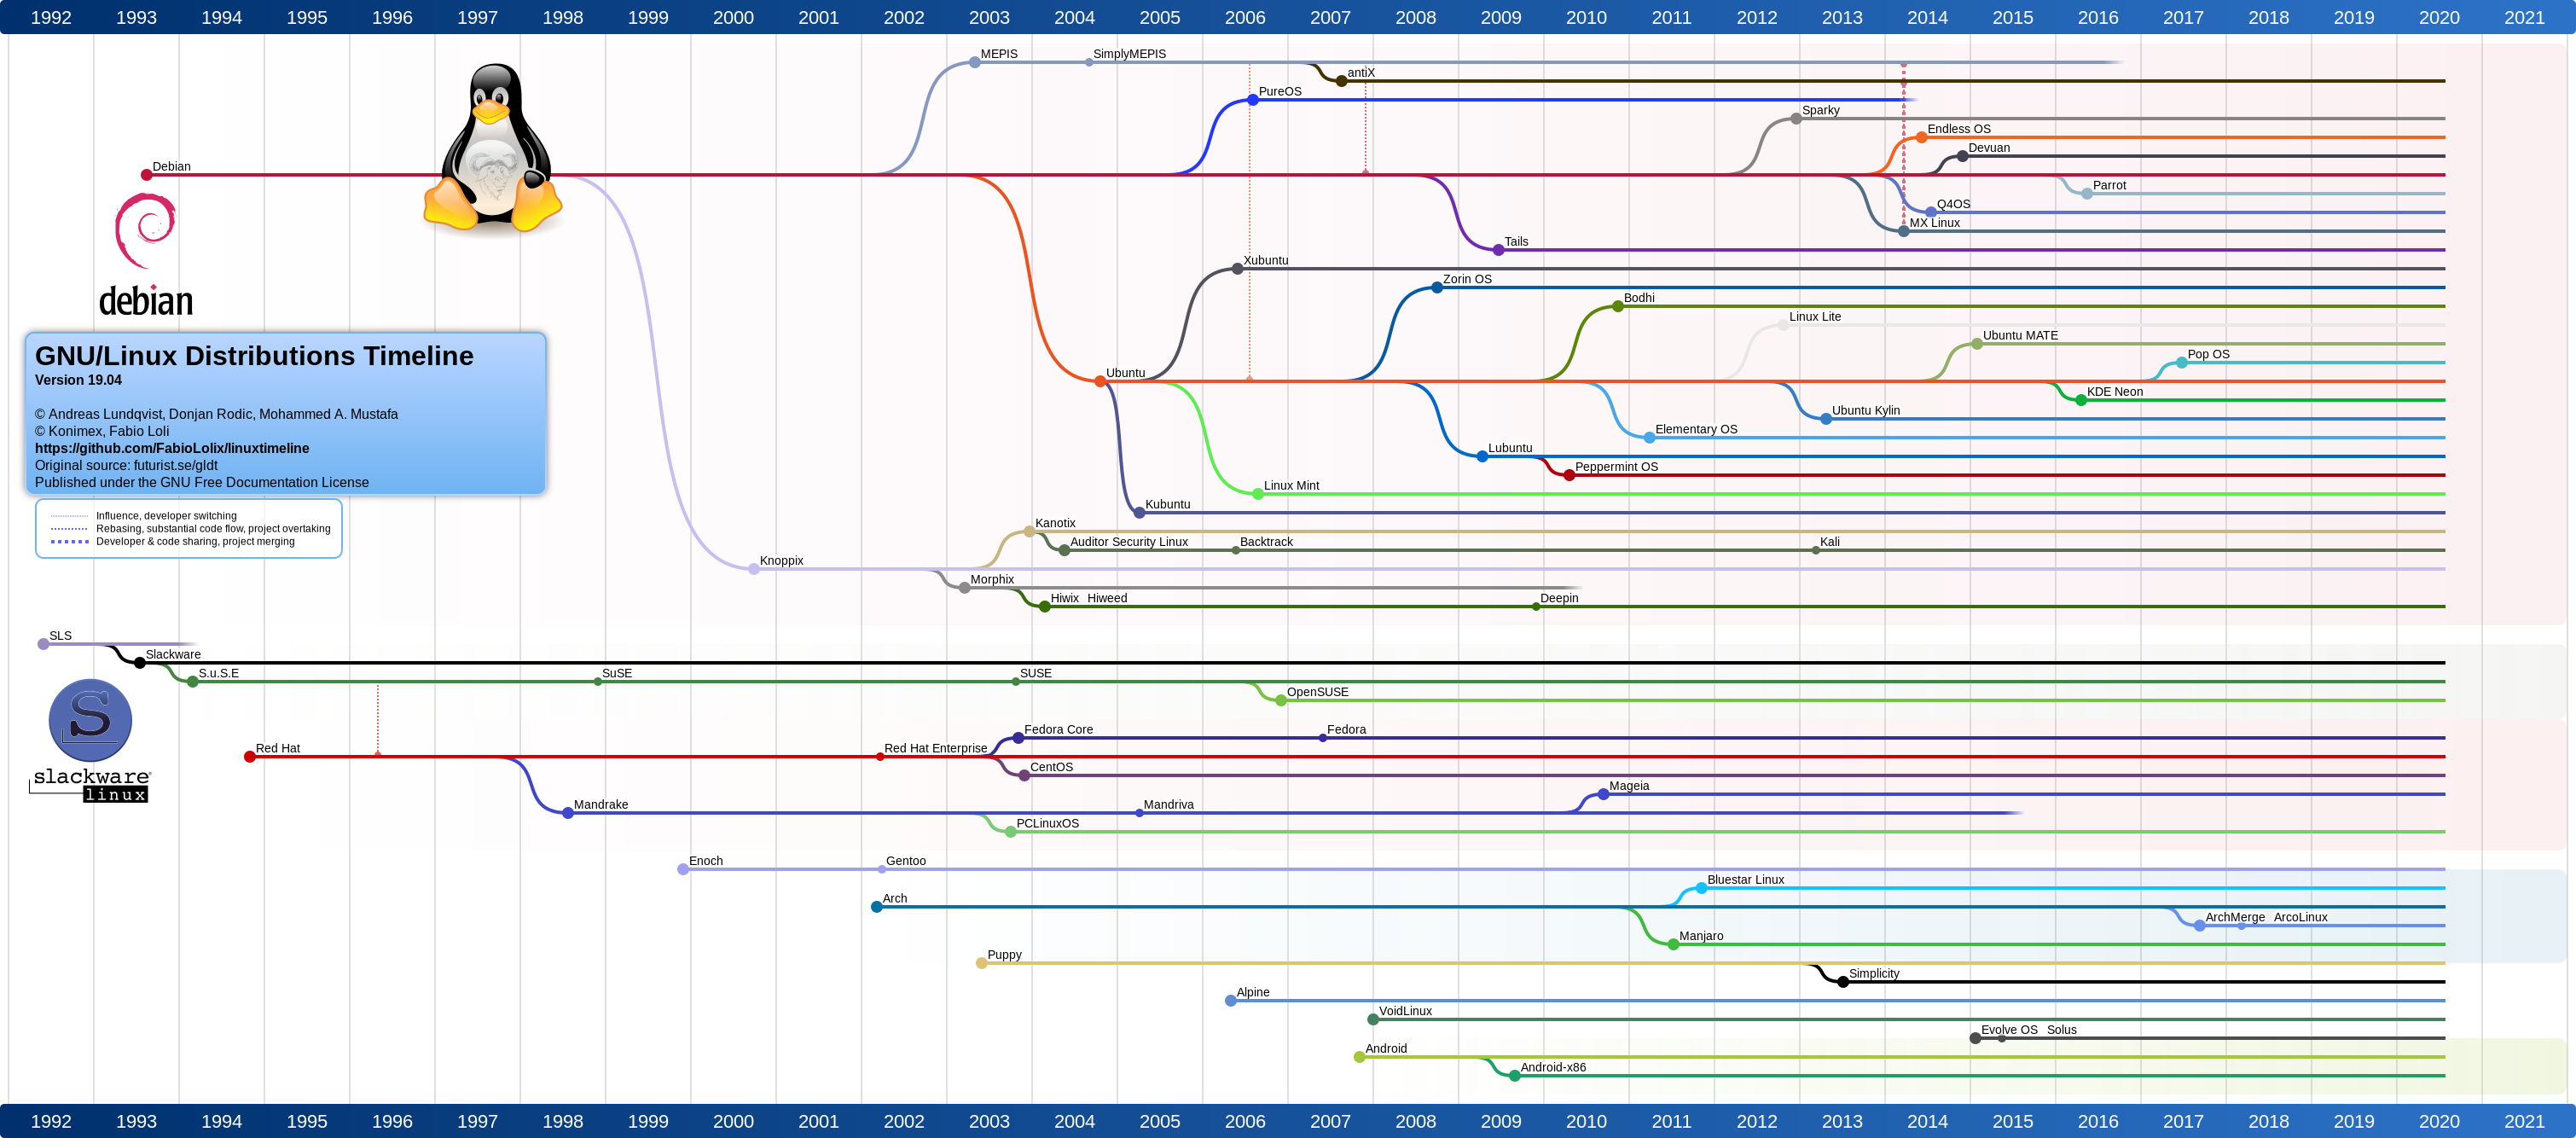
\includegraphics[height=1.7in,width=4.0in,viewport=0 0 2400 1080,clip]{Figures/Linux_distro-timeline.png}
%\caption{\textrm{The wave-particle duality and Photoelectric effect}}
\label{Linux-distri-timeline}
\end{figure}
}
%\section{虚拟机与\rm{Linux}的安装}
\section{\rm{Linux}命令简介}
\frame
{
	\frametitle{与目录和文件有关的命令}
	\begin{itemize}
\setlength{\itemsep}{-10pt}
		\item \textcolor{blue}{mkdir}:~创建目录
\begin{figure}[h!]
\centering
\vspace{-11.5pt}
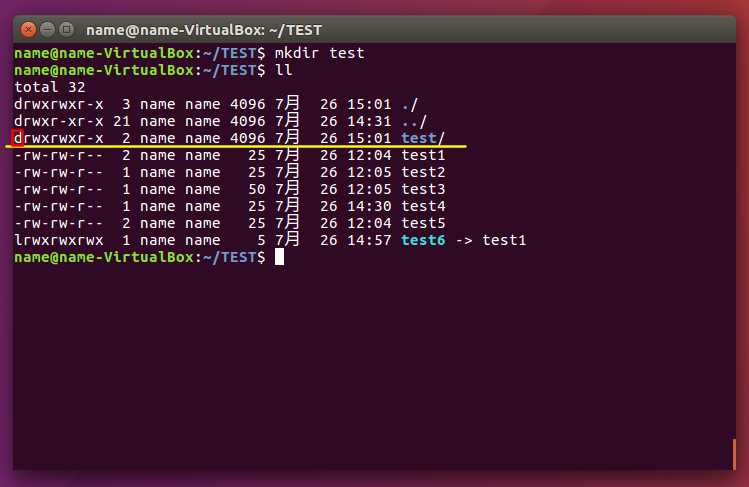
\includegraphics[height=1.2in,width=3.9in,viewport=0 220 800 470,clip]{Figures/Ubuntu-mkdir.png}
%\caption{\textrm{The wave-particle duality and Photoelectric effect}}
\label{Linux-command-mkdir}
\end{figure}
		\item \textcolor{blue}{cd}:~改变工作目录
\begin{figure}[h!]
\centering
\vspace{-9.5pt}
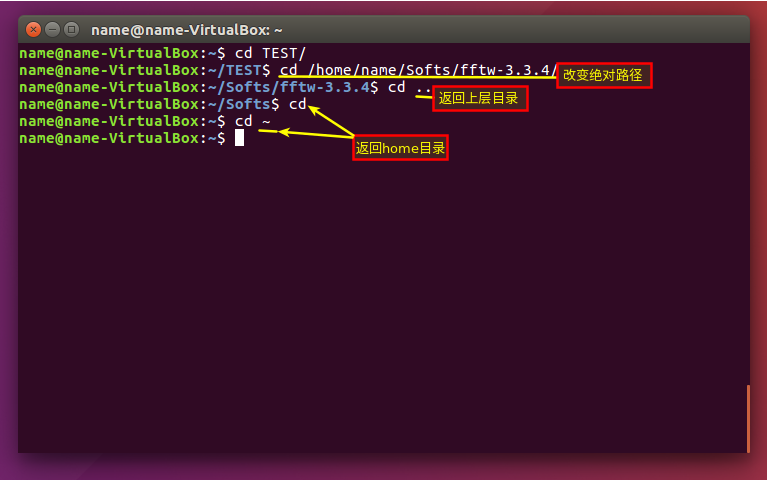
\includegraphics[height=0.8in,width=3.9in,viewport=0 310 800 470,clip]{Figures/Ubuntu-cd.png}
%\caption{\textrm{The wave-particle duality and Photoelectric effect}}
\label{Linux-command-cd}
\end{figure}
	\end{itemize}
}

\frame
{
	\frametitle{与目录和文件有关的命令}
	\begin{itemize}
		\item \textcolor{blue}{chmod}:~改变工作目录的权限
\begin{figure}[h!]
\centering
\vspace{-9.5pt}
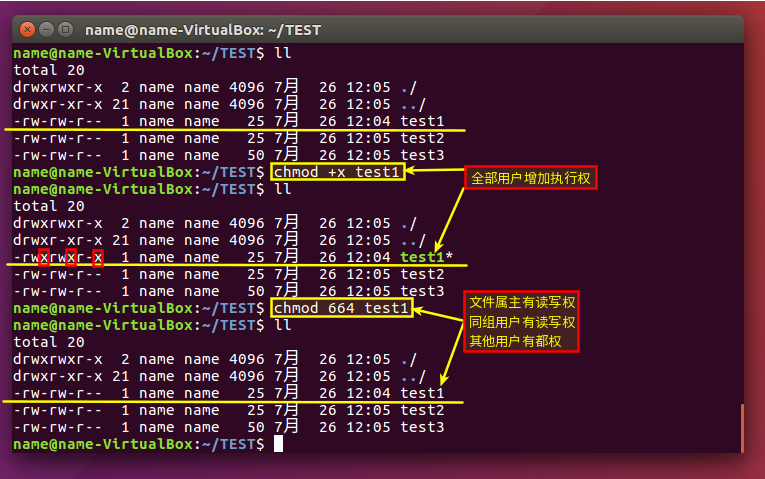
\includegraphics[height=2.3in,width=3.9in,viewport=0 0 800 470,clip]{Figures/Ubuntu-chmod.png}
%\caption{\textrm{The wave-particle duality and Photoelectric effect}}
\label{Linux-command-chmod}
\end{figure}
	\end{itemize}
}

\frame
{
	\frametitle{与目录和文件有关的命令}
	\begin{itemize}
		\item \textcolor{blue}{chown}:~改变文件的属主
\begin{figure}[h!]
\centering
\vspace{-2.5pt}
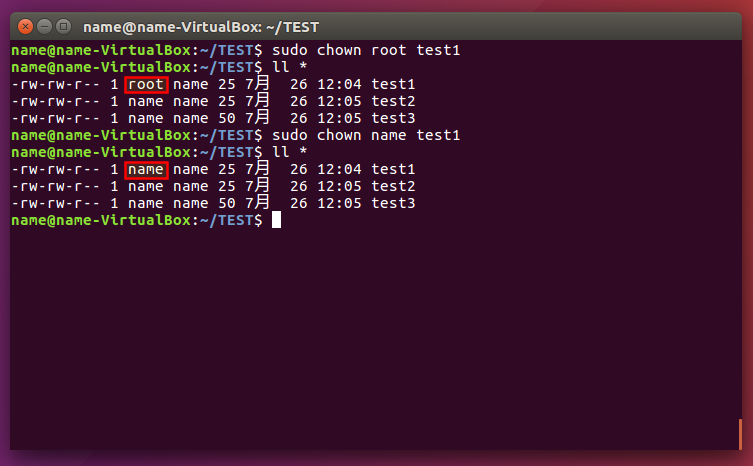
\includegraphics[height=2.1in,width=3.9in,viewport=0 70 800 470,clip]{Figures/Ubuntu-chown.png}
%\caption{\textrm{The wave-particle duality and Photoelectric effect}}
\label{Linux-command-chown}
\end{figure}
	\end{itemize}
}

\frame
{
	\frametitle{与目录和文件有关的命令}
	\begin{itemize}
		\item \textcolor{blue}{cp}:~将文件\textrm{copy}到另一个文件或另一目录
\begin{figure}[h!]
\centering
\vspace{-2.5pt}
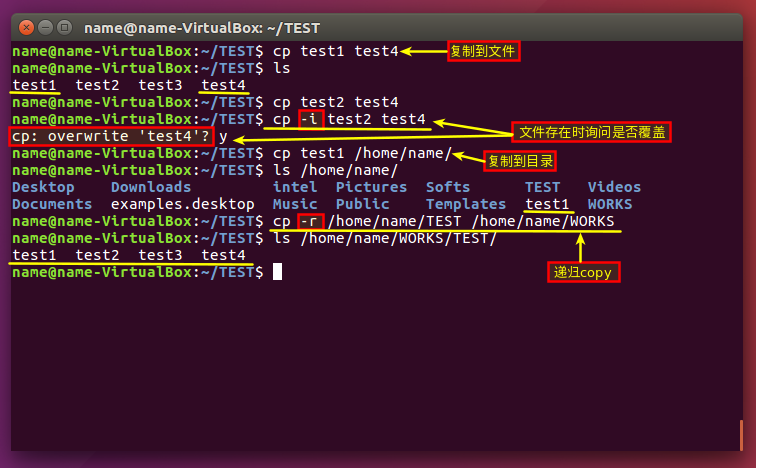
\includegraphics[height=2.2in,width=3.9in,viewport=0 0 800 470,clip]{Figures/Ubuntu-cp.png}
%\caption{\textrm{The wave-particle duality and Photoelectric effect}}
\label{Linux-command-cp}
\end{figure}
	\end{itemize}
}

\frame
{
	\frametitle{与目录和文件有关的命令}
	\begin{itemize}
\setlength{\itemsep}{-10pt}
		\item \textcolor{blue}{diff}:~逐行比较两个文件,列出不同
\begin{figure}[h!]
\centering
\vspace{-11.5pt}
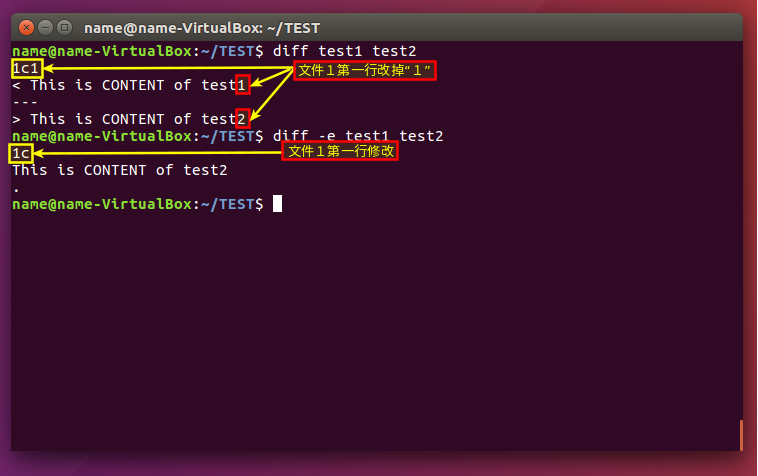
\includegraphics[height=1.0in,width=3.9in,viewport=0 250 800 470,clip]{Figures/Ubuntu-diff.png}
%\caption{\textrm{The wave-particle duality and Photoelectric effect}}
\label{Linux-command-diff}
\end{figure}
		\item \textcolor{blue}{find}:~搜索文件\textrm{(\textcolor{magenta}{文件所在位置检索})}
\begin{figure}[h!]
\centering
\vspace{-11.5pt}
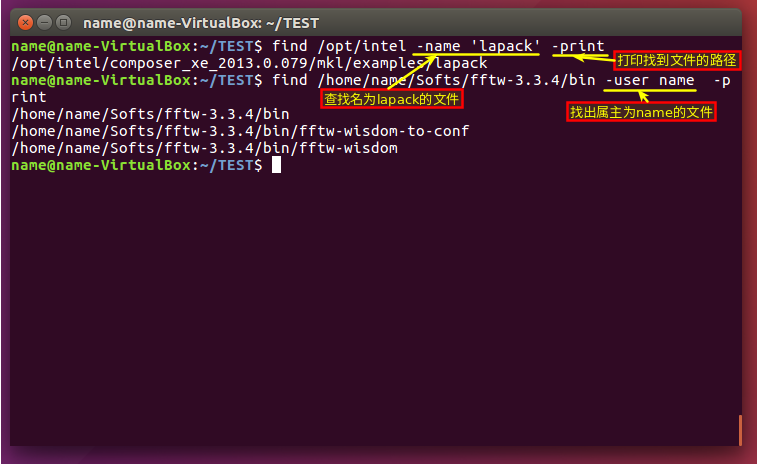
\includegraphics[height=1.0in,width=3.9in,viewport=0 270 800 470,clip]{Figures/Ubuntu-find.png}
%\caption{\textrm{The wave-particle duality and Photoelectric effect}}
\label{Linux-command-find}
\end{figure}
\end{itemize}
}

\frame
{
	\frametitle{与目录和文件有关的命令}
	\begin{itemize}
\setlength{\itemsep}{-10pt}
		\item \textcolor{blue}{grep}:~按给定模式搜索文件\textrm{(\textcolor{magenta}{文件所含内容搜索})}
\begin{figure}[h!]
\centering
\vspace{-12.5pt}
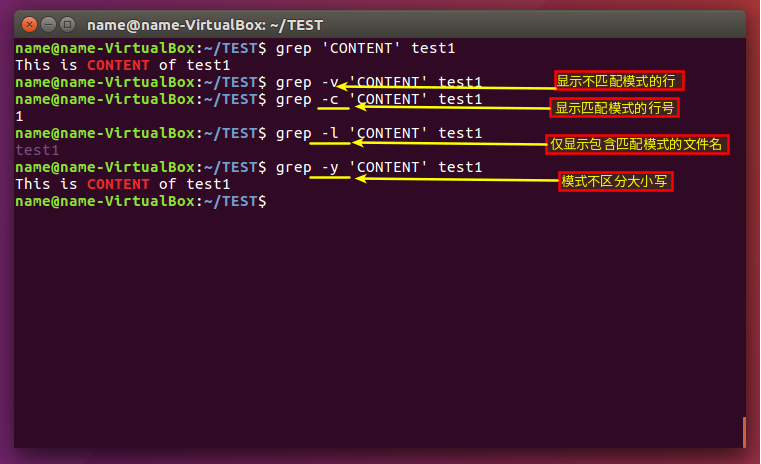
\includegraphics[height=1.0in,width=3.9in,viewport=0 250 800 470,clip]{Figures/Ubuntu-grep.png}
%\caption{\textrm{The wave-particle duality and Photoelectric effect}}
\label{Linux-command-grep}
\end{figure}
		\item \textcolor{blue}{head}:~显示指定文件前若干行
\begin{figure}[h!]
\centering
\vspace{-12.5pt}
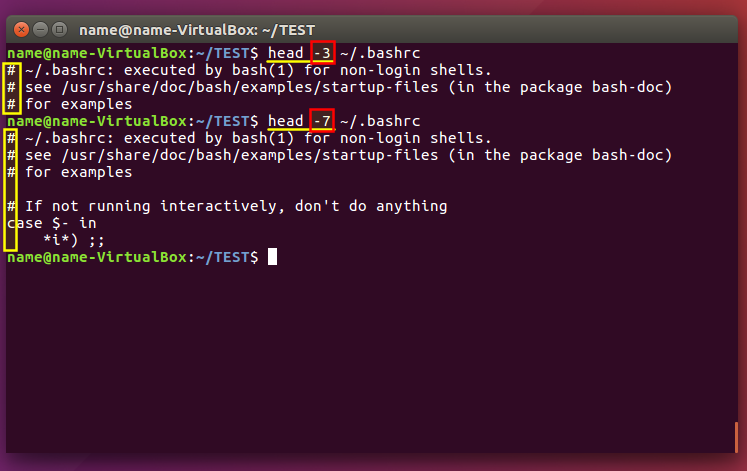
\includegraphics[height=1.2in,width=3.9in,viewport=0 200 800 470,clip]{Figures/Ubuntu-head.png}
%\caption{\textrm{The wave-particle duality and Photoelectric effect}}
\label{Linux-command-head}
\end{figure}
\end{itemize}
}

\frame
{
	\frametitle{与目录和文件有关的命令}
	\begin{itemize}
		\item \textcolor{blue}{ln}:~建立文件链接\textrm{(link)}
\begin{figure}[h!]
\centering
\vspace{-18.5pt}
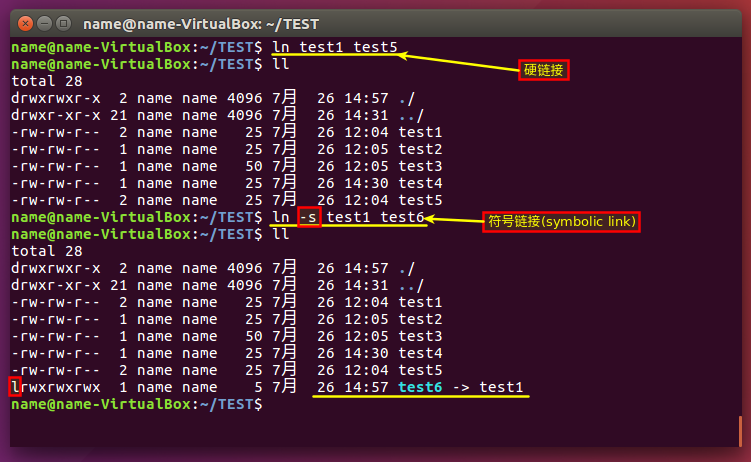
\includegraphics[height=2.0in,width=3.8in,viewport=0 50 800 470,clip]{Figures/Ubuntu-ln.png}
%\caption{\textrm{The wave-particle duality and Photoelectric effect}}
\label{Linux-command-ln}
\end{figure}
\vspace{-18.5pt}
\textcolor{red}{注意1:}~\textcolor{blue}{cp~-r}~会将链接文件\textrm{copy}成独立文件,如果需要保护文件符号链接\textrm{(软链接)}属性,建议用\textcolor{blue}{tar}命令\\
\textcolor{red}{注意2:}~不在同一文件系统\textrm{(如位于不同磁盘分区)}中的文件只能用符号链接,不能用硬链接
	\end{itemize}
}

\frame
{
	\frametitle{与目录和文件有关的命令}
	\begin{itemize}
		\item \textcolor{blue}{ls}:~列出目录中的内容
\begin{figure}[h!]
\centering
\vspace{-2.5pt}
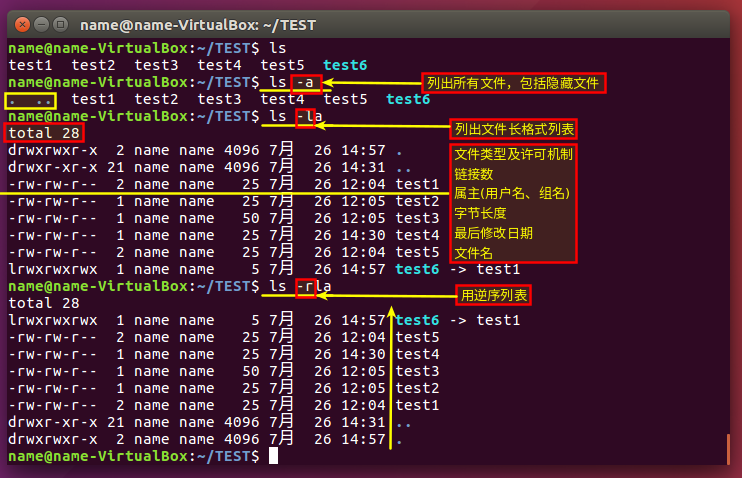
\includegraphics[height=2.2in,width=3.9in,viewport=0 0 800 470,clip]{Figures/Ubuntu-ls.png}
%\caption{\textrm{The wave-particle duality and Photoelectric effect}}
\label{Linux-command-ls}
\end{figure}
	\end{itemize}
}

\frame
{
	\frametitle{与目录和文件有关的命令}
\begin{minipage}{0.58\textwidth}
\begin{itemize}
	\item \textcolor{blue}{more:}~分屏显示信息
\begin{figure}[h!]
\centering
\hspace*{-32.5pt}
\vspace{-18.5pt}
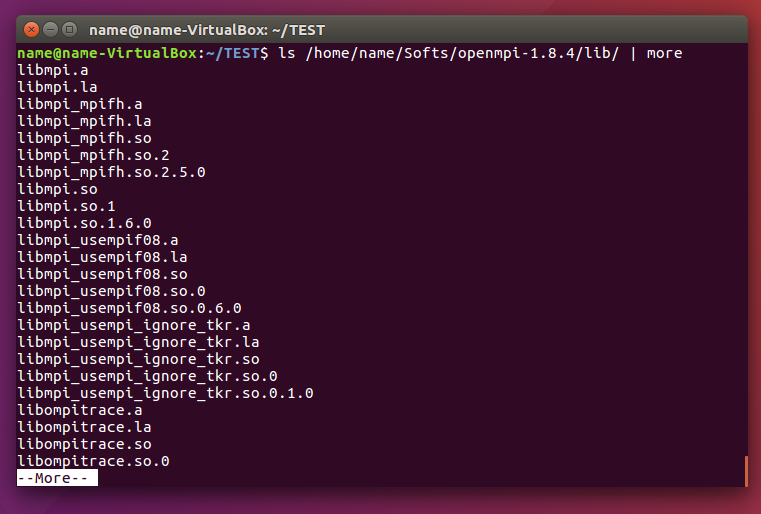
\includegraphics[height=1.8in,width=2.7in,viewport=0 0 800 500,clip]{Figures/Ubuntu-more.png}
%\caption{\textrm{The wave-particle duality and Photoelectric effect}}
\label{Linux-command-more}
\end{figure}
	\end{itemize}
\end{minipage}
\begin{minipage}{0.38\textwidth}
	\begin{itemize}
		\item \textcolor{brown}{-c}~清屏而非滚屏
		\item \textcolor{brown}{-f}~遇长行不折回
		\item \textrm{i}空格~显示后续\textrm{i}行
		\item \textrm{q}或\textrm{Q}~退出\textcolor{blue}{more}
		\item \textrm{=}~显示当前行号
		\item \textrm{h}~帮助信息
	\end{itemize}
\end{minipage}
}

\frame
{
	\frametitle{与目录和文件有关的命令}
	\begin{itemize}
		\item \textcolor{blue}{mv}:~文件或目录的移动或更名
\begin{figure}[h!]
\centering
\vspace{-12.5pt}
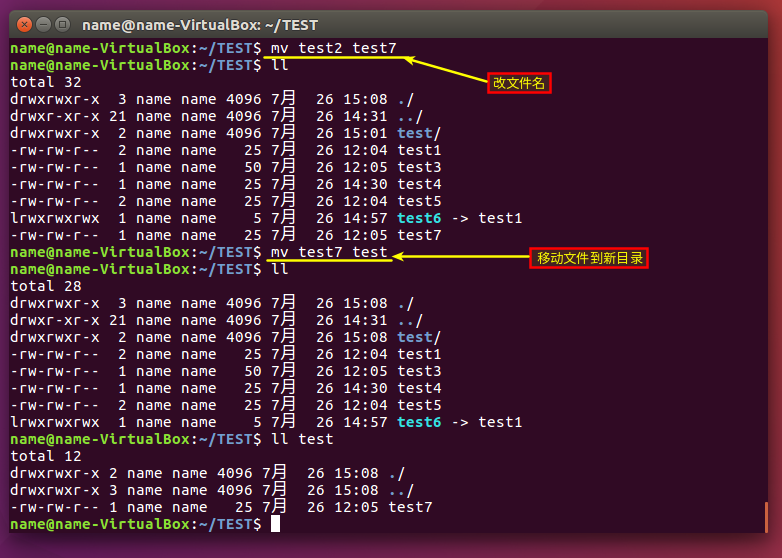
\includegraphics[height=2.3in,width=3.9in,viewport=0 0 800 550,clip]{Figures/Ubuntu-mv.png}
%\caption{\textrm{The wave-particle duality and Photoelectric effect}}
\label{Linux-command-mv}
\end{figure}
	\end{itemize}
}

\frame
{
	\frametitle{与目录和文件有关的命令}
	\begin{itemize}
\setlength{\itemsep}{-10pt}
		\item \textcolor{blue}{pwd}:~显示当前目录绝对路径
\begin{figure}[h!]
\centering
\vspace{-15.5pt}
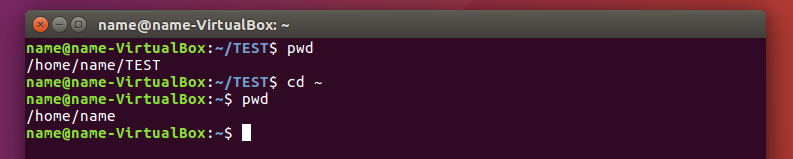
\includegraphics[height=0.6in,width=3.9in,viewport=0 0 800 160,clip]{Figures/Ubuntu-pwd.png}
%\caption{\textrm{The wave-particle duality and Photoelectric effect}}
\label{Linux-command-pwd}
\end{figure}
		\item \textcolor{blue}{rm}:~删除文件或目录
\begin{figure}[h!]
\centering
\vspace{-15.5pt}
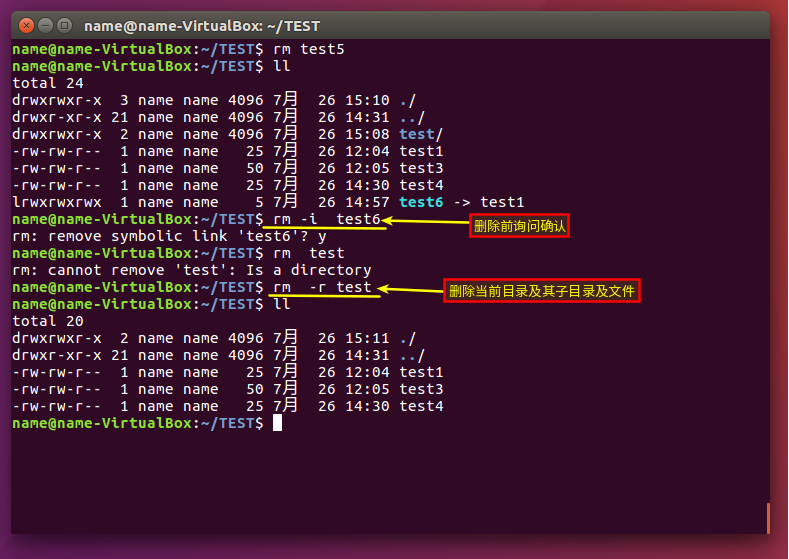
\includegraphics[height=1.7in,width=3.9in,viewport=0 120 800 550,clip]{Figures/Ubuntu-rm.png}
%\caption{\textrm{The wave-particle duality and Photoelectric effect}}
\label{Linux-command-rm}
\end{figure}
\end{itemize}
}

\frame
{
	\frametitle{与目录和文件有关的命令}
\begin{minipage}{0.48\textwidth}
\begin{itemize}
	\item \textcolor{blue}{sort:}~对指定文件按行排序
\begin{figure}[h!]
\centering
\hspace*{-28.5pt}
\vspace{18.5pt}
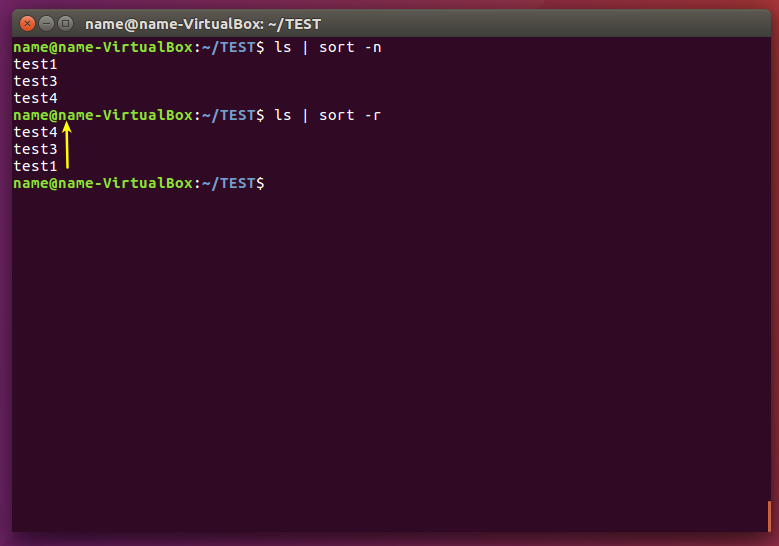
\includegraphics[height=1.3in,width=2.1in,viewport=0 350 400 600,clip]{Figures/Ubuntu-sort.png}
%\caption{\textrm{The wave-particle duality and Photoelectric effect}}
\label{Linux-command-sort}
\end{figure}
	\end{itemize}
\end{minipage}
\begin{minipage}{0.50\textwidth}
	\begin{itemize}
		\item \textcolor{brown}{-b}~忽略开头的空格和制表符
		\item \textcolor{brown}{-d}~仅字母、数字、空格按字典排序
		\item \textcolor{brown}{-f}~不区分字母大小写
		\item \textcolor{brown}{-n}~按数字升序排列
		\item \textcolor{brown}{-r}~按当前顺序的逆序排序
		\item \textcolor{brown}{-u}~忽略重复行
		\item \textcolor{brown}{-o}~指定输出文件名
	\end{itemize}
\end{minipage}
}

\frame
{
	\frametitle{与目录和文件有关的命令}
	\begin{itemize}
		\item \textcolor{blue}{tail}:~显示指定文件的最后部分
\begin{figure}[h!]
\centering
\vspace{-12.5pt}
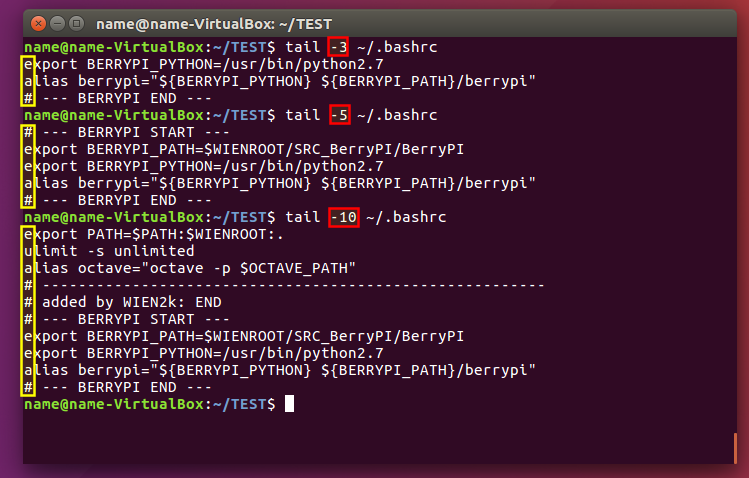
\includegraphics[height=2.3in,width=3.9in,viewport=0 0 800 480,clip]{Figures/Ubuntu-tail.png}
%\caption{\textrm{The wave-particle duality and Photoelectric effect}}
\label{Linux-command-tail}
\end{figure}
	\end{itemize}
}

\frame
{
	\frametitle{与目录和文件有关的命令}
	\begin{itemize}
		\item \textcolor{blue}{tar}:~将若干文件存档或读取存档文件
\begin{figure}[h!]
\centering
\vspace{-12.5pt}
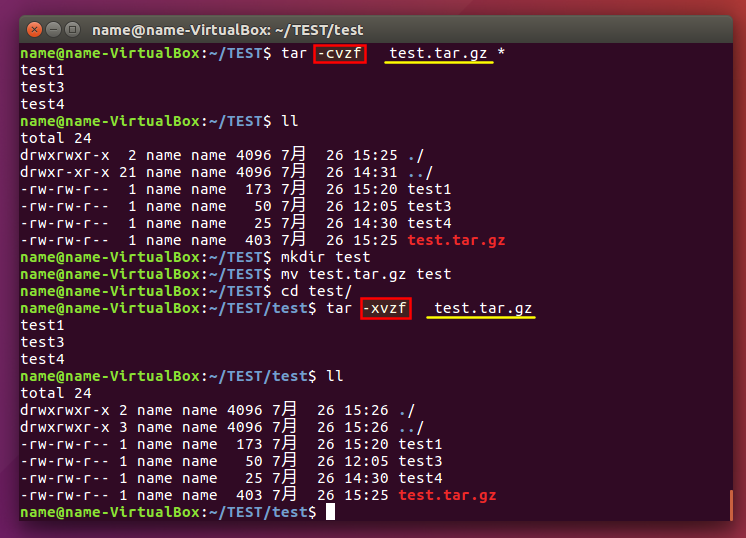
\includegraphics[height=2.3in,width=3.9in,viewport=0 10 800 530,clip]{Figures/Ubuntu-tar.png}
%\caption{\textrm{The wave-particle duality and Photoelectric effect}}
\label{Linux-command-tar}
\end{figure}
	\end{itemize}
}

\frame
{
	\frametitle{与目录和文件有关的命令}
	\begin{itemize}
		\item \textcolor{blue}{wc}:~统计指定文件的行数、词数和字符数
\begin{figure}[h!]
\centering
\vspace{-12.5pt}
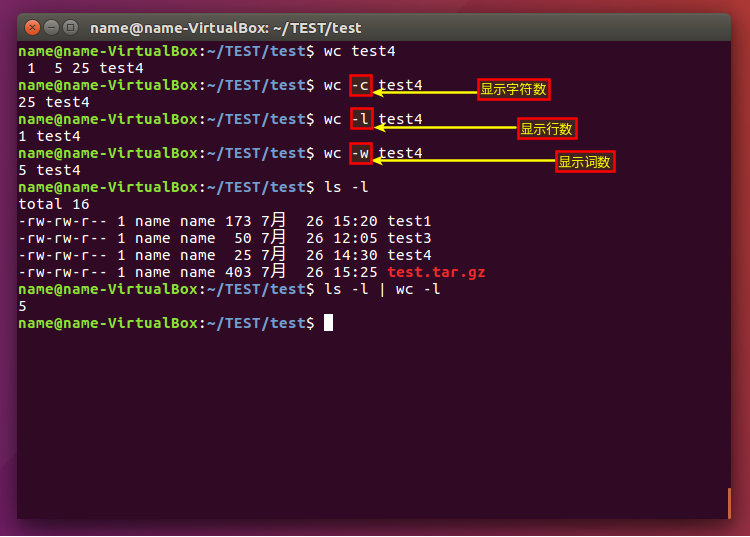
\includegraphics[height=2.3in,width=3.9in,viewport=0 60 800 560,clip]{Figures/Ubuntu-wc.png}
%\caption{\textrm{The wave-particle duality and Photoelectric effect}}
\label{Linux-command-wc}
\end{figure}
	\end{itemize}
}

\frame
{
	\frametitle{状态信息查询命令}
	\begin{itemize}
\setlength{\itemsep}{-10pt}
		\item \textcolor{blue}{date}:~显示日期与时间
\begin{figure}[h!]
\centering
\vspace{-15.5pt}
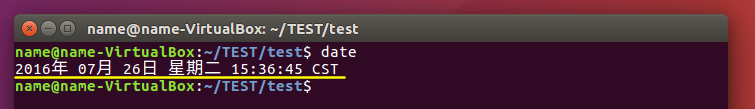
\includegraphics[height=0.6in,width=3.9in,viewport=0 0 800 130,clip]{Figures/Ubuntu-date.png}
%\caption{\textrm{The wave-particle duality and Photoelectric effect}}
\label{Linux-command-date}
\end{figure}
		\item \textcolor{blue}{df}:~查询磁盘空间使用情况
\begin{figure}[h!]
\centering
\vspace{-15.5pt}
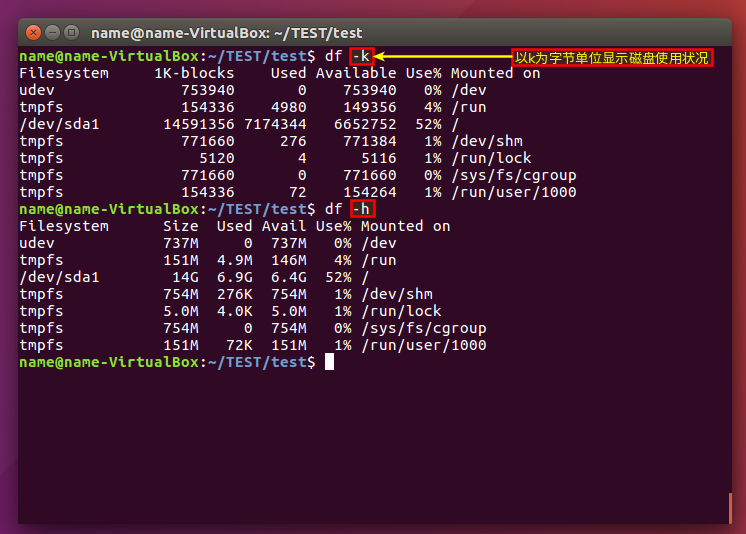
\includegraphics[height=1.7in,width=3.9in,viewport=0 150 800 530,clip]{Figures/Ubuntu-df.png}
%\caption{\textrm{The wave-particle duality and Photoelectric effect}}
\label{Linux-command-df}
\end{figure}
\end{itemize}
}

\frame
{
	\frametitle{状态信息查询命令}
	\begin{itemize}
		\item \textcolor{blue}{du}:~统计目录或文件所占磁盘空间的大小
\begin{figure}[h!]
\centering
\vspace{-5.5pt}
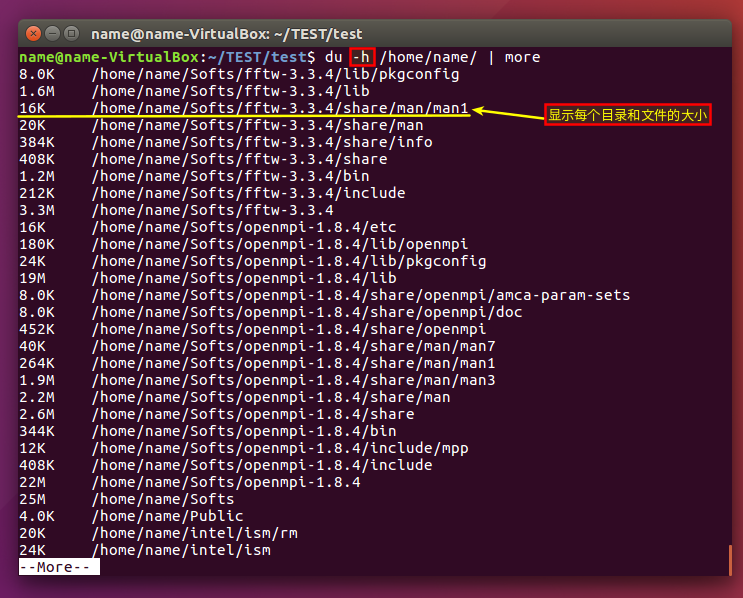
\includegraphics[height=2.1in,width=3.6in,viewport=0 0 800 580,clip]{Figures/Ubuntu-du-1.png}
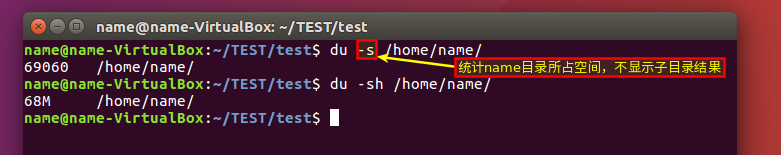
\includegraphics[height=0.6in,width=3.7in,viewport=0 0 880 150,clip]{Figures/Ubuntu-du-2.png}
%\caption{\textrm{The wave-particle duality and Photoelectric effect}}
\label{Linux-command-du}
\end{figure}
	\end{itemize}
}

\frame
{
	\frametitle{状态信息查询命令}
	\begin{itemize}
\setlength{\itemsep}{-15pt}
		\item \textcolor{blue}{ps}:~检查进程状态
\begin{figure}[h!]
\centering
\vspace{-10.5pt}
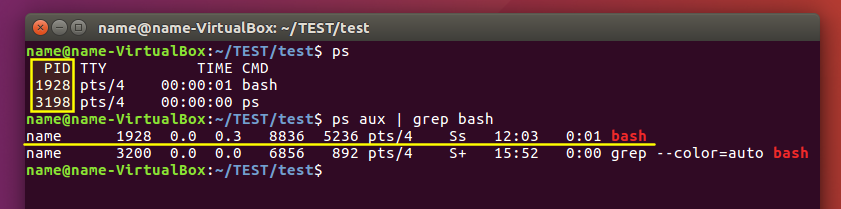
\includegraphics[height=0.9in,width=3.7in,viewport=0 20 850 230,clip]{Figures/Ubuntu-ps.png}
%\caption{\textrm{The wave-particle duality and Photoelectric effect}}
\label{Linux-command-ps}
\end{figure}
		\item \textcolor{blue}{time}:~统计程序或命令运行的时间
\begin{figure}[h!]
\centering
\vspace{-5.5pt}
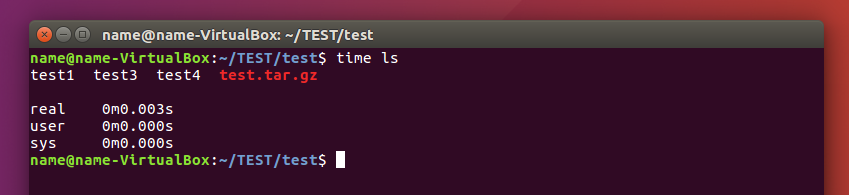
\includegraphics[height=0.7in,width=3.7in,viewport=0 20 850 180,clip]{Figures/Ubuntu-time.png}
%\caption{\textrm{The wave-particle duality and Photoelectric effect}}
\label{Linux-command-time}
\end{figure}
		\item \textcolor{blue}{w}:~检查状态状态
\begin{figure}[h!]
\centering
\vspace{-18.5pt}
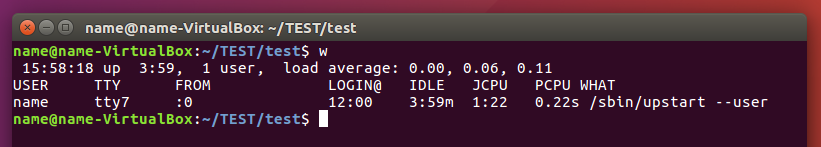
\includegraphics[height=0.7in,width=3.8in,viewport=0 0 850 150,clip]{Figures/Ubuntu-w.png}
%\caption{\textrm{The wave-particle duality and Photoelectric effect}}
\label{Linux-command-w}
\end{figure}
\end{itemize}
}

\frame
{
	\frametitle{状态信息查询命令}
	\begin{itemize}
		\item \textcolor{blue}{whereis}:~确定命令位置
		\item \textcolor{blue}{which}:~确定命令位置
		\item \textcolor{blue}{who}:~列出正在使用系统的用户
		\item \textcolor{blue}{whoami}:~显示正在使用本终端的用户名
	\end{itemize}
\begin{figure}[h!]
\centering
\vspace{-5.5pt}
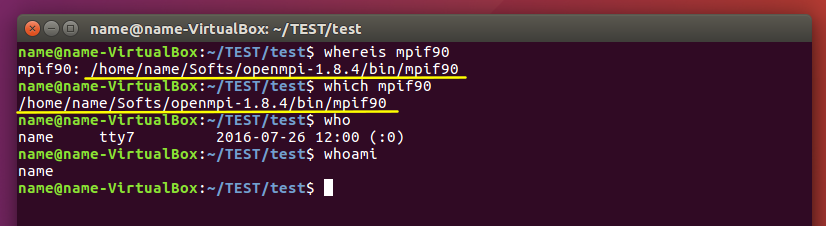
\includegraphics[height=1.4in,width=3.9in,viewport=0 30 800 300,clip]{Figures/Ubuntu-which.png}
%\caption{\textrm{The wave-particle duality and Photoelectric effect}}
\label{Linux-command-which}
\end{figure}
}

\frame
{
	\frametitle{网络查询命令}
	\begin{itemize}
		\item \textcolor{blue}{whereis}:~确定命令位置
		\item \textcolor{blue}{which}:~确定命令位置
		\item \textcolor{blue}{who}:~列出正在使用系统的用户
		\item \textcolor{blue}{whoami}:~显示正在使用本终端的用户名
	\end{itemize}
\begin{figure}[h!]
\centering
\vspace{-5.5pt}
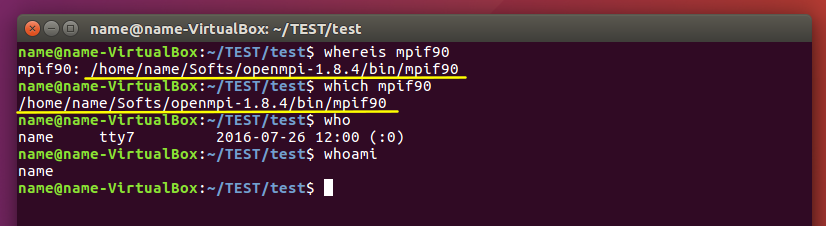
\includegraphics[height=1.4in,width=3.9in,viewport=0 30 800 300,clip]{Figures/Ubuntu-which.png}
%\caption{\textrm{The wave-particle duality and Photoelectric effect}}
\label{Linux-command-which}
\end{figure}
}



\section{\rm{Linux}下的软件安装与\rm{Make}}
\frame
{
	\frametitle{软件编译的一般过程}
高级语言编写的程序,从源代码变成可执行的文件,必须经过完整的编译(\textrm{compilation})过程,共有四个步骤
\begin{figure}[h!]
	\vskip -8pt
\centering
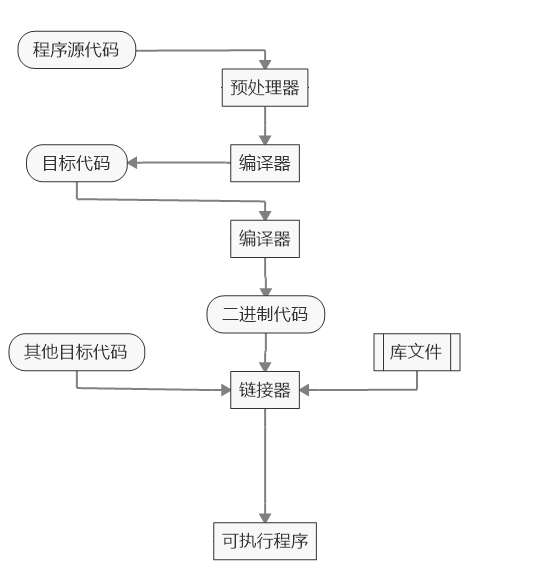
\includegraphics[height=2.5in,viewport=0 0 500 600,clip]{Figures/compiler_procedure.png}
%\includegraphics[height=1.8in,width=4.in,viewport=30 210 570 440,clip]{PAW_projector.eps}
\caption{\small \textrm{软件编译的步骤示意(预编译-编译-汇编-链接).}}%(与文献\cite{EPJB33-47_2003}图1对比)
\label{Fig:Compiler}
\end{figure}
编译的功能类似于翻译,把人类编写的符合高级语言语法规则的语句,翻译成计算机可以执行的指令。
}

\frame
{
	\frametitle{软件编译的一般过程}
\begin{itemize}
	\item 预处理\textrm{(Pre-Processing)}:~将根据源代码中以字符\#开头的指令要求,用预处理器\textrm{cpp}修改原始程序\\
		如\textrm{C}程序中\textcolor{purple}{\textrm{\#include <stdio.h>}}指令告诉预处理器读系统头文件\textrm{stdio.h}的内容,并把它直接插入到程序文本中去,得到另外一个\textrm{C}程序%通常是 以.i作为文件扩展名的。
	\item 编译\textrm{(Compiling)}:~在编译阶段,编译器\textrm{compiler}会检查代码的规范性
		\begin{enumerate}
			\item 检查源代码是否存在拼写和语法错误等,检查无误后,编译器将把代码翻译成汇编语言
			\item 确定代码实际执行的具体任务和指令
		\end{enumerate}
		汇编语言为不同高级语言不同编译器提供了通用的语言。比如\textrm{C}编译器和\textrm{Fortran}编译器产生的输出文件用的都是一样的汇编语言

		用户可以使用\textrm{-S}选项来进行查看,该选项只完成编译过程而不进行汇编
\end{itemize}
}

\frame
{
	\frametitle{软件编译的一般过程}
\begin{itemize}
	\item 汇编\textrm{(Assembling)}:~汇编阶段是把编译阶段生成的\textrm{.s}文件(汇编代码)转成目标文件\\
		用户可使用\textrm{-c}选项就可看到汇编代码将转化为\textrm{.o}的二进制目标代码
	\item 链接\textrm{(Linking)}:~汇编生成二进制代码之后,就进入了链接阶段\\
完成了链接之后,编译器就可以生成最终可执行文件
		%用户采用高级语言编写的程序中,有相当一部分功能是由外部软件函数库或其他目标代码提供,无需用户自行编写(如输入输出命令、复杂函数的解法器等),因此程序执行时就需要和这些函数库的支持
\end{itemize}

		函数库一般分为静态库(后缀名一般为\textrm{.a})和动态库(后缀名一般为\textrm{.so})两种
		\begin{itemize}
			\item \textcolor{blue}{静态库}是指编译链接时,把库文件的代码全部加入到可执行文件中,因此生成的文件比较大,但在运行时就不再需要库文件支持
			\item \textcolor{blue}{动态库}在编译链接时并没有把库文件的代码加入到可执行文件中,而在程序执行时由运行时链接文件加载库,这样可以节省系统的开销
		\end{itemize}
}

\frame
{
	\frametitle{\textrm{Linux}的软件编译:~\textcolor{purple}{\textbf{Make}}}
	\textcolor{blue}{\textbf{make}}是一个命令工具,它通过解释\textrm{Makefile}文件中的指令,完成对软件的编译、链接和执行
	\begin{itemize}
		\item 在\textrm{Linux}环境下使用\textrm{GNU}软件,\textcolor{blue}{\textbf{make}}是重要的编译命令和工具,能够帮助用户比较容易地构建一个属于自己的软件工程
		\item 理解\textcolor{blue}{\textbf{make}}方式安装软件的核心就是学会\textrm{Makefile}文件的编写\\
			\textrm{Makefile}文件是 \textcolor{blue}{\textbf{make}} 正常工作的基础。在\textrm{Makefile}文件中描述了整个工程所有文件的编译顺序、编译规则
	\end{itemize}
	使用\textcolor{blue}{\textbf{make}}工具编译软件时,有几种文件在执行\textcolor{blue}{\textbf{make}}时会被编译或重新编译
	\begin{enumerate}
		\item 所有源文件没有被编译过的,将对各源文件进行编译并进行链接,生成最后的可执行程序
		\item 每个上次执行\textcolor{blue}{\textbf{make}}后修改过的源代码文件在本次执行\textcolor{blue}{\textbf{make}}时会被重新编译
		\item 如果头文件在上次执行\textcolor{blue}{\textbf{make}}后被修改,则所有包含此头文件的源文件在本次执\textcolor{blue}{\textbf{make}}时将会被重新编译
	\end{enumerate}
}

\frame
{
	\frametitle{\textrm{Makefile}文件的编写规则}
	一个简单的\textrm{Makefile}描述规则的组成格式:
	\begin{displaymath}
		\mathrm{TARGET}\cdots : \mathrm{PREREQUISITES}\cdots
	\end{displaymath}
	\begin{displaymath}
		\begin{matrix}
			&\textrm{COMMAND}\\
			&\cdots\\
			&\cdots
		\end{matrix}
	\end{displaymath}

	\begin{itemize}
		\item \textcolor{blue}{\textrm{target}}:~规则的目标\\
			目标通常是最后需要生成的文件名或者为了实现编译过程中必要的中间过程文件名,可以是.o文件、也可以是最后的可执行程序的文件名等\\
			目标也可以是一个\textcolor{blue}{\textbf{make}}执行的动作的名称\\ 
			如目标\textcolor{magenta}{\textrm{clean}}就不是一个文件,仅表示执行一个动作的标识,这样的目标也称为“伪目标”
	\end{itemize}
}

\frame
{
	\frametitle{\textrm{Makefile}文件的编写规则}
	\begin{itemize}
		\item \textcolor{blue}{\textrm{prerequisites}}:~规则的依赖\\
			生成规则目标所需要的文件名列表,通常一个目标依赖于一个或者多个文件

		\item \textcolor{blue}{\textrm{command}}:~规则的命令行\\
			规则所要执行的动作(可以是任意的\textrm{shell}命令或者是可在\textrm{shell}下执行的程序)\\
			命令行限定了\textcolor{blue}{\textbf{make}}执行该规则时所需要的动作
	\end{itemize}

	一个\textrm{Makefile}中的每个规则可以包含多个命令行,每条命令占一行

	\vskip 8pt
	\textcolor{red}{注意}:~每一个命令行必须以[\textrm{Tab}]字符开始
\vskip 5pt
	\textrm{[Tab]}字符告诉\textcolor{blue}{\textbf{make}}此行是命令行,\textcolor{blue}{\textbf{make}}按命令完成相应的动作
}

\frame
{
	\frametitle{通过\textcolor{purple}{\textbf{make}}~运行\textrm{Makefile}}
	\begin{itemize}
		\item 对于一般用户来说,\textcolor{blue}{\textbf{make}}命令像命令行参数一样接收目标
		\item 当\textcolor{blue}{\textbf{make}}命令第一次执行时,它扫描\textrm{Makefile}找到目标以及其依赖(如果这些依赖自身也是目标,继续为这些依赖扫描\textrm{Makefile} 建立其依赖关系,然后编译
		\item 一旦主依赖编译之后,然后编译主目标(通过 \textcolor{blue}{\textbf{make}}命令传入)\\
			默认情况下,\textcolor{blue}{\textbf{make}}执行的是\textrm{Makefile}中的第一个规则,此规则的第一个目标称之为“最终目的”或者“终极目标”(就是一个\textrm{Makefile}最终需要更新或者创建的目标)
		\item 假设用户对某个源文件进行了修改,再次执行 \textcolor{blue}{\textbf{make}}命令,将只编译与该源文件相关的目标文件
	\end{itemize}
	采用\textcolor{blue}{\textbf{make}}编译并获得最终的可执行文件,有可能节省大量的时间
}

\frame
{
	\frametitle{\textcolor{purple}{\textbf{make}}~执行举例}
	假定程序的源代码为如下结构
\begin{figure}[h!]
	\vskip -3pt
\centering
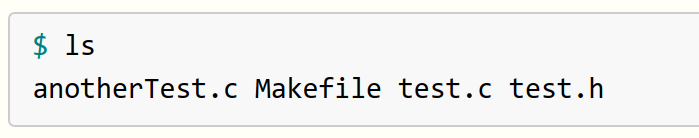
\includegraphics[height=0.4in,clip]{Figures/Make_Makefile_1.png}
%\includegraphics[height=1.8in,width=4.in,viewport=30 210 570 440,clip]{PAW_projector.eps}
%\caption{\small \textrm{软件编译的步骤示意(预编译-编译-汇编-链接).}}%(与文献\cite{EPJB33-47_2003}图1对比)
\label{Fig:Make_Makefile_1}
\end{figure}
其中\textrm{Makefile}的内容如下
\begin{figure}[h!]
	\vskip -4pt
\centering
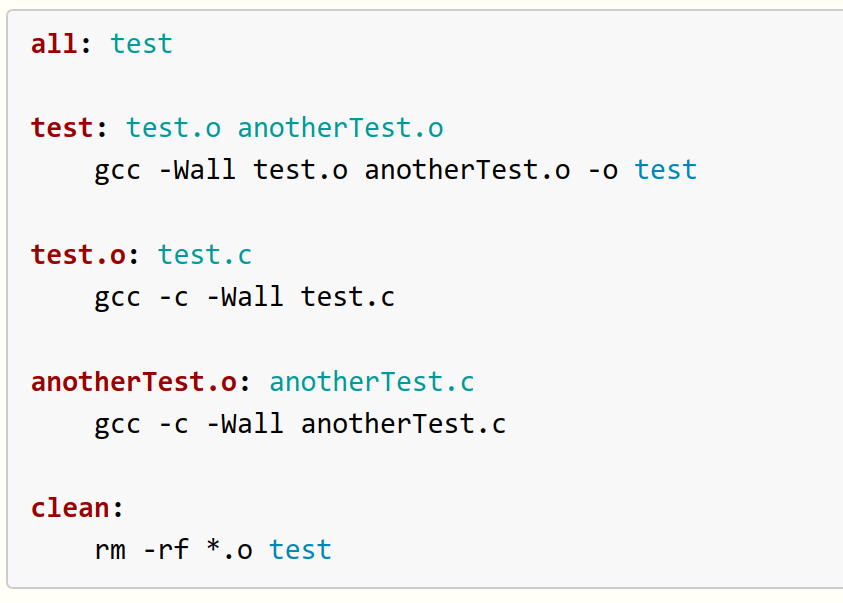
\includegraphics[height=2.0in,clip]{Figures/Make_Makefile_2.png}
%\includegraphics[height=1.8in,width=4.in,viewport=30 210 570 440,clip]{PAW_projector.eps}
%\caption{\small \textrm{软件编译的步骤示意(预编译-编译-汇编-链接).}}%(与文献\cite{EPJB33-47_2003}图1对比)
\label{Fig:Make_Makefile_2}
\end{figure}
}

\frame
{
	\frametitle{\textcolor{purple}{\textbf{make}}~执行举例}
	初次执行\textcolor{blue}{\textbf{make}}命令
\begin{figure}[h!]
	\vskip -3pt
\centering
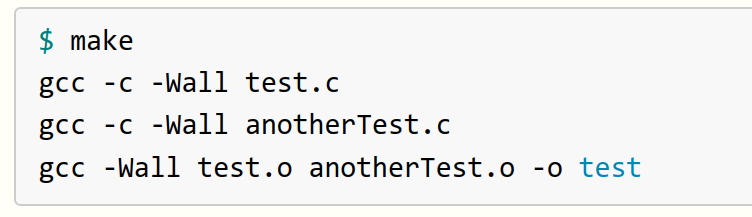
\includegraphics[height=0.9in,clip]{Figures/Make_Makefile_3.png}
%\includegraphics[height=1.8in,width=4.in,viewport=30 210 570 440,clip]{PAW_projector.eps}
%\caption{\small \textrm{软件编译的步骤示意(预编译-编译-汇编-链接).}}%(与文献\cite{EPJB33-47_2003}图1对比)
\label{Fig:Make_Makefile_3}
\end{figure}
再次查看该目录下的内容,将会发现里面多了一些 \textrm{.o} 文件和可执行文件\textcolor{green}{\textrm{test}}
\begin{figure}[h!]
	\vskip -3pt
\centering
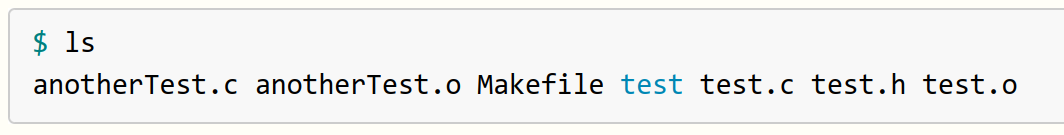
\includegraphics[height=0.4in,clip]{Figures/Make_Makefile_4.png}
%\includegraphics[height=1.8in,width=4.in,viewport=30 210 570 440,clip]{PAW_projector.eps}
%\caption{\small \textrm{软件编译的步骤示意(预编译-编译-汇编-链接).}}%(与文献\cite{EPJB33-47_2003}图1对比)
\label{Fig:Make_Makefile_4}
\end{figure}
}

\frame
{
	\frametitle{\textcolor{purple}{\textbf{make}}~执行举例}
	如果用户对源代码\textrm{test.c}作一些改动,再次执行\textcolor{blue}{\textbf{make}}命令
\begin{figure}[h!]
	\vskip -3pt
\centering
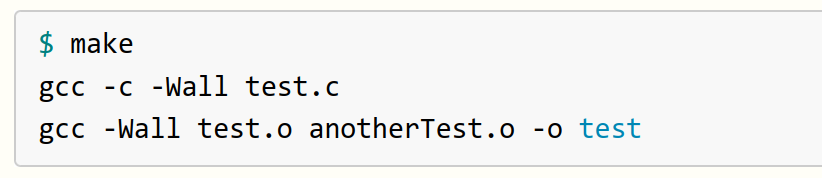
\includegraphics[height=0.7in,clip]{Figures/Make_Makefile_5.png}
%\includegraphics[height=1.8in,width=4.in,viewport=30 210 570 440,clip]{PAW_projector.eps}
%\caption{\small \textrm{软件编译的步骤示意(预编译-编译-汇编-链接).}}%(与文献\cite{EPJB33-47_2003}图1对比)
\label{Fig:Make_Makefile_5}
\end{figure}
可以看到,只有\textrm{test.o} 被重新编译,而另一个 \textrm{anotherTest.o} 并未重新编译

最后,用户如果需要清理所有的目标文件和可执行文件\textrm{test},可以使用目标 \textcolor{magenta}{\textrm{clean}}:
\begin{figure}[h!]
	\vskip -4pt
\centering
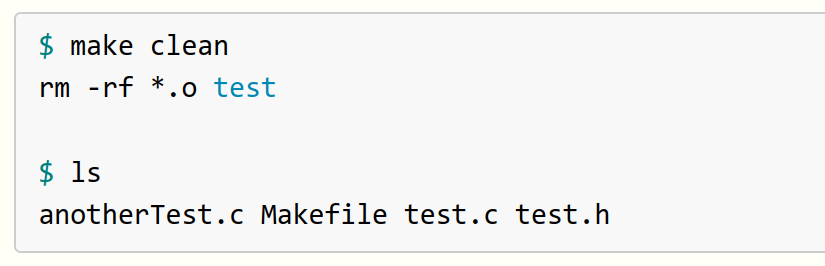
\includegraphics[height=0.8in,clip]{Figures/Make_Makefile_6.png}
%\includegraphics[height=1.8in,width=4.in,viewport=30 210 570 440,clip]{PAW_projector.eps}
%\caption{\small \textrm{软件编译的步骤示意(预编译-编译-汇编-链接).}}%(与文献\cite{EPJB33-47_2003}图1对比)
\label{Fig:Make_Makefile_6}
\end{figure}
可以看到所有的\textrm{.o}文件和可执行文件 \textcolor{green}{\textrm{test}}都已被删除
}

\frame
{
	\frametitle{\textcolor{purple}{\textbf{make}}~的常用可选参数}
	为适应编译过程中的复杂需要,\textcolor{blue}{\textbf{make}}工具还提供了一些选项,以满足用户在编译时的不同需求。这里介绍几个常见的可选项
	\begin{itemize}
		\item 默认的\textcolor{blue}{\textbf{make}}命令不会编译那些自从上次编译之后就没有更改的文件,但如果想覆盖\textcolor{blue}{\textbf{make}}这种默认行为,可以使用 \textrm{-B} 选项
\begin{figure}[h!]
	\vskip -4pt
\centering
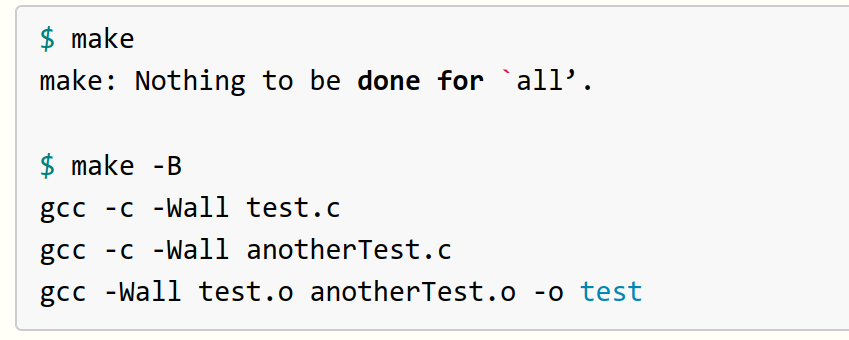
\includegraphics[height=1.3in,clip]{Figures/Make_Makefile_7.png}
%\includegraphics[height=1.8in,width=4.in,viewport=30 210 570 440,clip]{PAW_projector.eps}
%\caption{\small \textrm{软件编译的步骤示意(预编译-编译-汇编-链接).}}%(与文献\cite{EPJB33-47_2003}图1对比)
\label{Fig:Make_Makefile_7}
\end{figure}
	\end{itemize}
}

\frame
{
	\frametitle{\textcolor{purple}{\textbf{make}}~的常用可选参数}
	\begin{itemize}
\item 如果想将了解 \textcolor{blue}{\textbf{make}}执行时实际做了什么,可以使用 \textrm{-d} 选项
\begin{figure}[h!]
	\vskip -5pt
\centering
\includegraphics[height=2.6in,clip]{Figures/Make_Makefile_8.png}
%\includegraphics[height=1.8in,width=4.in,viewport=30 210 570 440,clip]{PAW_projector.eps}
%\caption{\small \textrm{软件编译的步骤示意(预编译-编译-汇编-链接).}}%(与文献\cite{EPJB33-47_2003}图1对比)
\label{Fig:Make_Makefile_8}
\end{figure}
	\end{itemize}
}

\frame
{
	\frametitle{\textcolor{purple}{\textbf{make}}~的常用可选参数}
	\begin{itemize}
\item 如果想让 \textcolor{blue}{\textbf{make}} 在查找 \textrm{Makefile}时切换到指定目录,可以使用 \textrm{-C} 选项\\
\vskip 5pt
	假设当前目录为
\begin{figure}[h!]
	\vskip -4pt
\centering
\includegraphics[height=0.6in,clip]{Figures/Make_Makefile_9-1.png}
%\includegraphics[height=1.8in,width=4.in,viewport=30 210 570 440,clip]{PAW_projector.eps}
%\caption{\small \textrm{软件编译的步骤示意(预编译-编译-汇编-链接).}}%(与文献\cite{EPJB33-47_2003}图1对比)
\label{Fig:Make_Makefile_9-1}
\end{figure}

\textcolor{blue}{\textbf{make}} 命令所执行的 \textrm{Makefile} 文件位于 \textrm{../make-dir/} 目录下
\begin{figure}[h!]
	\vskip -12pt
\centering
\includegraphics[height=0.8in,clip]{Figures/Make_Makefile_9-2.png}
%\includegraphics[height=1.8in,width=4.in,viewport=30 210 570 440,clip]{PAW_projector.eps}
%\caption{\small \textrm{软件编译的步骤示意(预编译-编译-汇编-链接).}}%(与文献\cite{EPJB33-47_2003}图1对比)
\label{Fig:Make_Makefile_9-2}
\end{figure}
	 \textcolor{blue}{\textbf{make}} 命令将先切到指定目录,执行完毕后再切换回当前目录
	\end{itemize}
}

\frame
{
	\frametitle{\textcolor{purple}{\textbf{make}}~的常用可选参数}
	\begin{itemize}
\item 如果想将 \textrm{Makefile} 文件重命名(这里取名为 \textrm{my\_makefile},也可是其它名),为了让 \textcolor{blue}{\textbf{make}} 仍将它也当成 \textrm{Makefile},可以使用 \textrm{-f} 选项
\begin{figure}[h!]
	\vskip -4pt
\centering
\includegraphics[height=0.4in,clip]{Figures/Make_Makefile_0.png}
%\includegraphics[height=1.8in,width=4.in,viewport=30 210 570 440,clip]{PAW_projector.eps}
%\caption{\small \textrm{软件编译的步骤示意(预编译-编译-汇编-链接).}}%(与文献\cite{EPJB33-47_2003}图1对比)
\label{Fig:Make_Makefile_0}
\end{figure}
\item \textrm{-h/--help}~显示帮助信息
\item \textrm{-i}~在执行时忽略所有的错误
\item \textrm{-j~[jobnumber]}~指定同时运行命令的个数\\
\vskip 3pt
	如果~\textrm{-j}~后没有\textrm{jobsnum}参数、\textcolor{blue}{\textbf{make}}运行命令时能运行多少就运行多少
	\end{itemize}
\vskip 3pt
\textcolor{blue}{\textbf{make}} 的可选参数还有很多,有关各选项的具体内容可运行命令\\
\textcolor{purple}{\textbf{man~make}}~ 查看
}

\frame[allowframebreaks]
{
	\frametitle{\textcolor{purple}{\textbf{make}}~的执行过程}
	\begin{itemize}
		\item 依次读取变量\$\{\textrm{MAKEFILES}\}定义的 \textrm{makefile} 文件列表
		\item 读取工作目录下的 \textrm{makefile}文件\\
			根据命名的查找默认顺序\textrm{GNUmakefile}, \textrm{makefile},\textrm{Makefile},首先找到哪个就读取哪个
		\item 依次读取工作目录 \textrm{makefile} 文件中使用指示符\textcolor{purple}{\textrm{include}}包含的文件
		\item 查找重建所有已读取的 \textrm{makefile} 文件的规则\\
			如果存在一个目标是当前读取的某一个 \textrm{makefile} 文件,则执行此规则重建此 \textrm{makefile} 文件,完成后从第一步开始重新执行
		\item 初始化变量值并展开那些需要立即展开的变量和函数并根据预设条件确定执行分支
		\item 根据“终极目标”以及其他目标的依赖关系建立依赖关系链表
		\item 执行除“终极目标”以外的所有的目标的规则\\
			规则中如果依赖文件中任一个 文件的时间戳比目标文件新,则使用规则所定义的命令重建目标文件
		\item 最后执行“终极目标”所在的规则
	\end{itemize}

	\vskip 15pt
	\textcolor{red}{总结}

	\textcolor{blue}{\textbf{make}}命令执行一个规则时的依据:\\
	\textcolor{red}{比较目标文件和所有的依赖文件的时间戳}
	\begin{itemize}
		\item 如果目标的时间戳比所有依赖文件的时间戳没有更新(依赖文件在上一次 \textcolor{blue}{\textbf{make}}命令执行之后没有被修改),那什么也不做;
		\item 否则(即依赖文件中的某一个或者全部在上一次\textcolor{blue}{\textbf{make}}命令执行后已经被修改过),规则定义的重建目标的命令将会被执行
	\end{itemize}

	这是\textcolor{blue}{\textbf{make}}命令工作的基础,也是其执行规制所定义命令的依据
}
